\subsection{Cosmic Radiation Methods}
\label{sec:Rad-Methods}

\subsection{Telemetry}
\label{sec:Telemetry}

All telemetry was handled via the RPi. The DB9 interface from the HASP Large Payload plate was converted to a 
RS-232 female plug. A Male RS 232 to Male USB \ref{fig:rs232-usb} was used to connect it to a USB port of the RPi. 
The downlink data packets were written to describe the radiation data. 
The uplink commands were sent to the RPi which delegated the work either to itself or the Arduino which 
was connected to the RPi via USB as shown in figure \ref{fig:telem-diagram}.

\begin{figure}[h!]
\centering
\begin{minipage}{.5\textwidth}
  \centering
  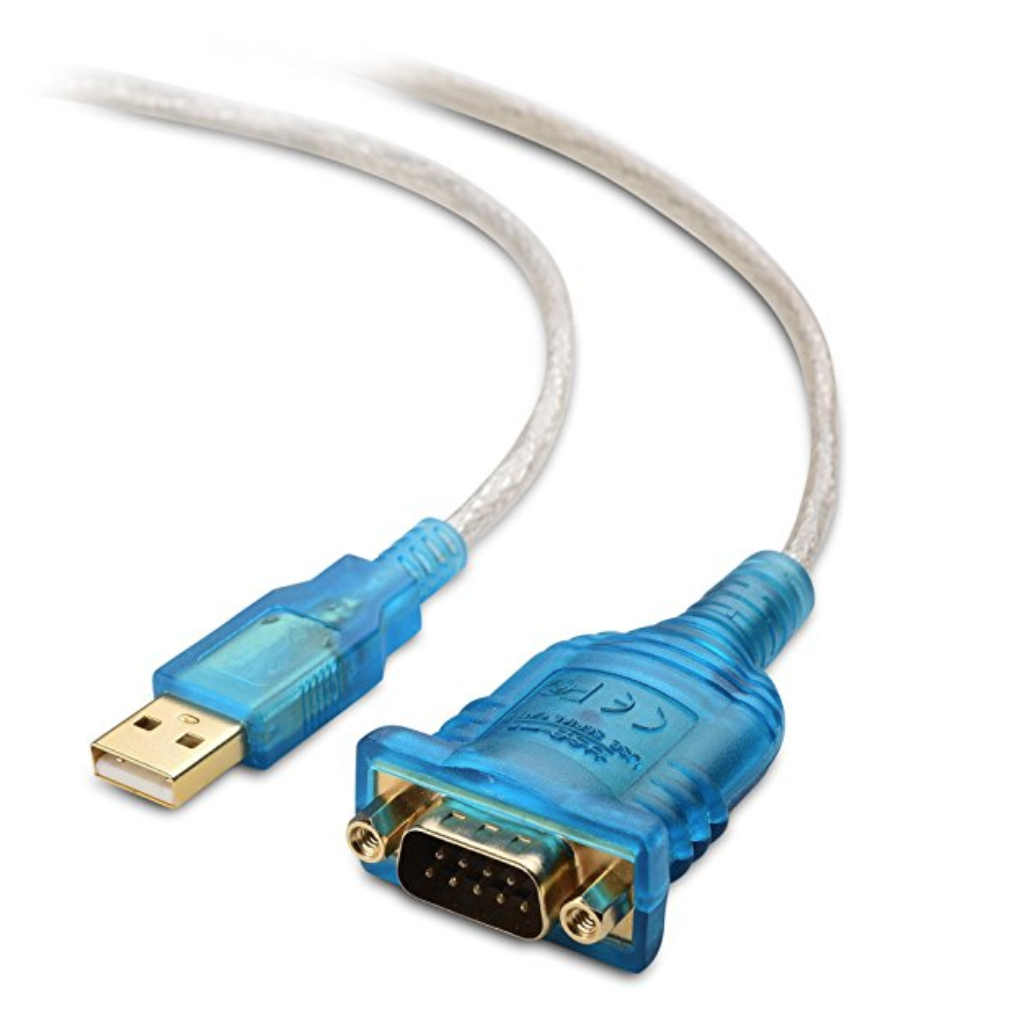
\includegraphics[width=.4\linewidth]{figures/rs232tousb.png}
  \caption{RS 232 to Male USB}{Cable used to connect the DB9 interface to the RPi}
  \label{fig:rs232tousb}
\end{minipage}%
\begin{minipage}{.5\textwidth}
  \centering
  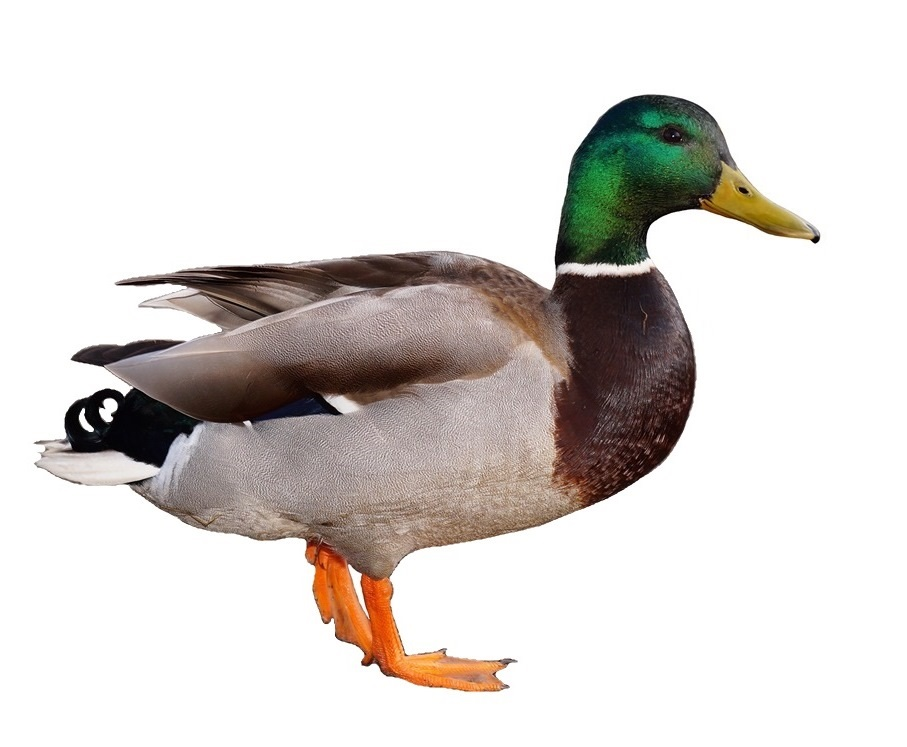
\includegraphics[width=.4\linewidth]{figures/duck.jpg}
  \caption{Telemetry}{Diagram depicting how telemetry was processed}
  \label{fig:telem-diagram}
\end{minipage}
\end{figure}

\subsubsection{Uplink}
\label{sec:Uplink} 


\subsubsection{Downlink}
\label{sec:Downlink}
